\begin{figure}[H]
	\centering
	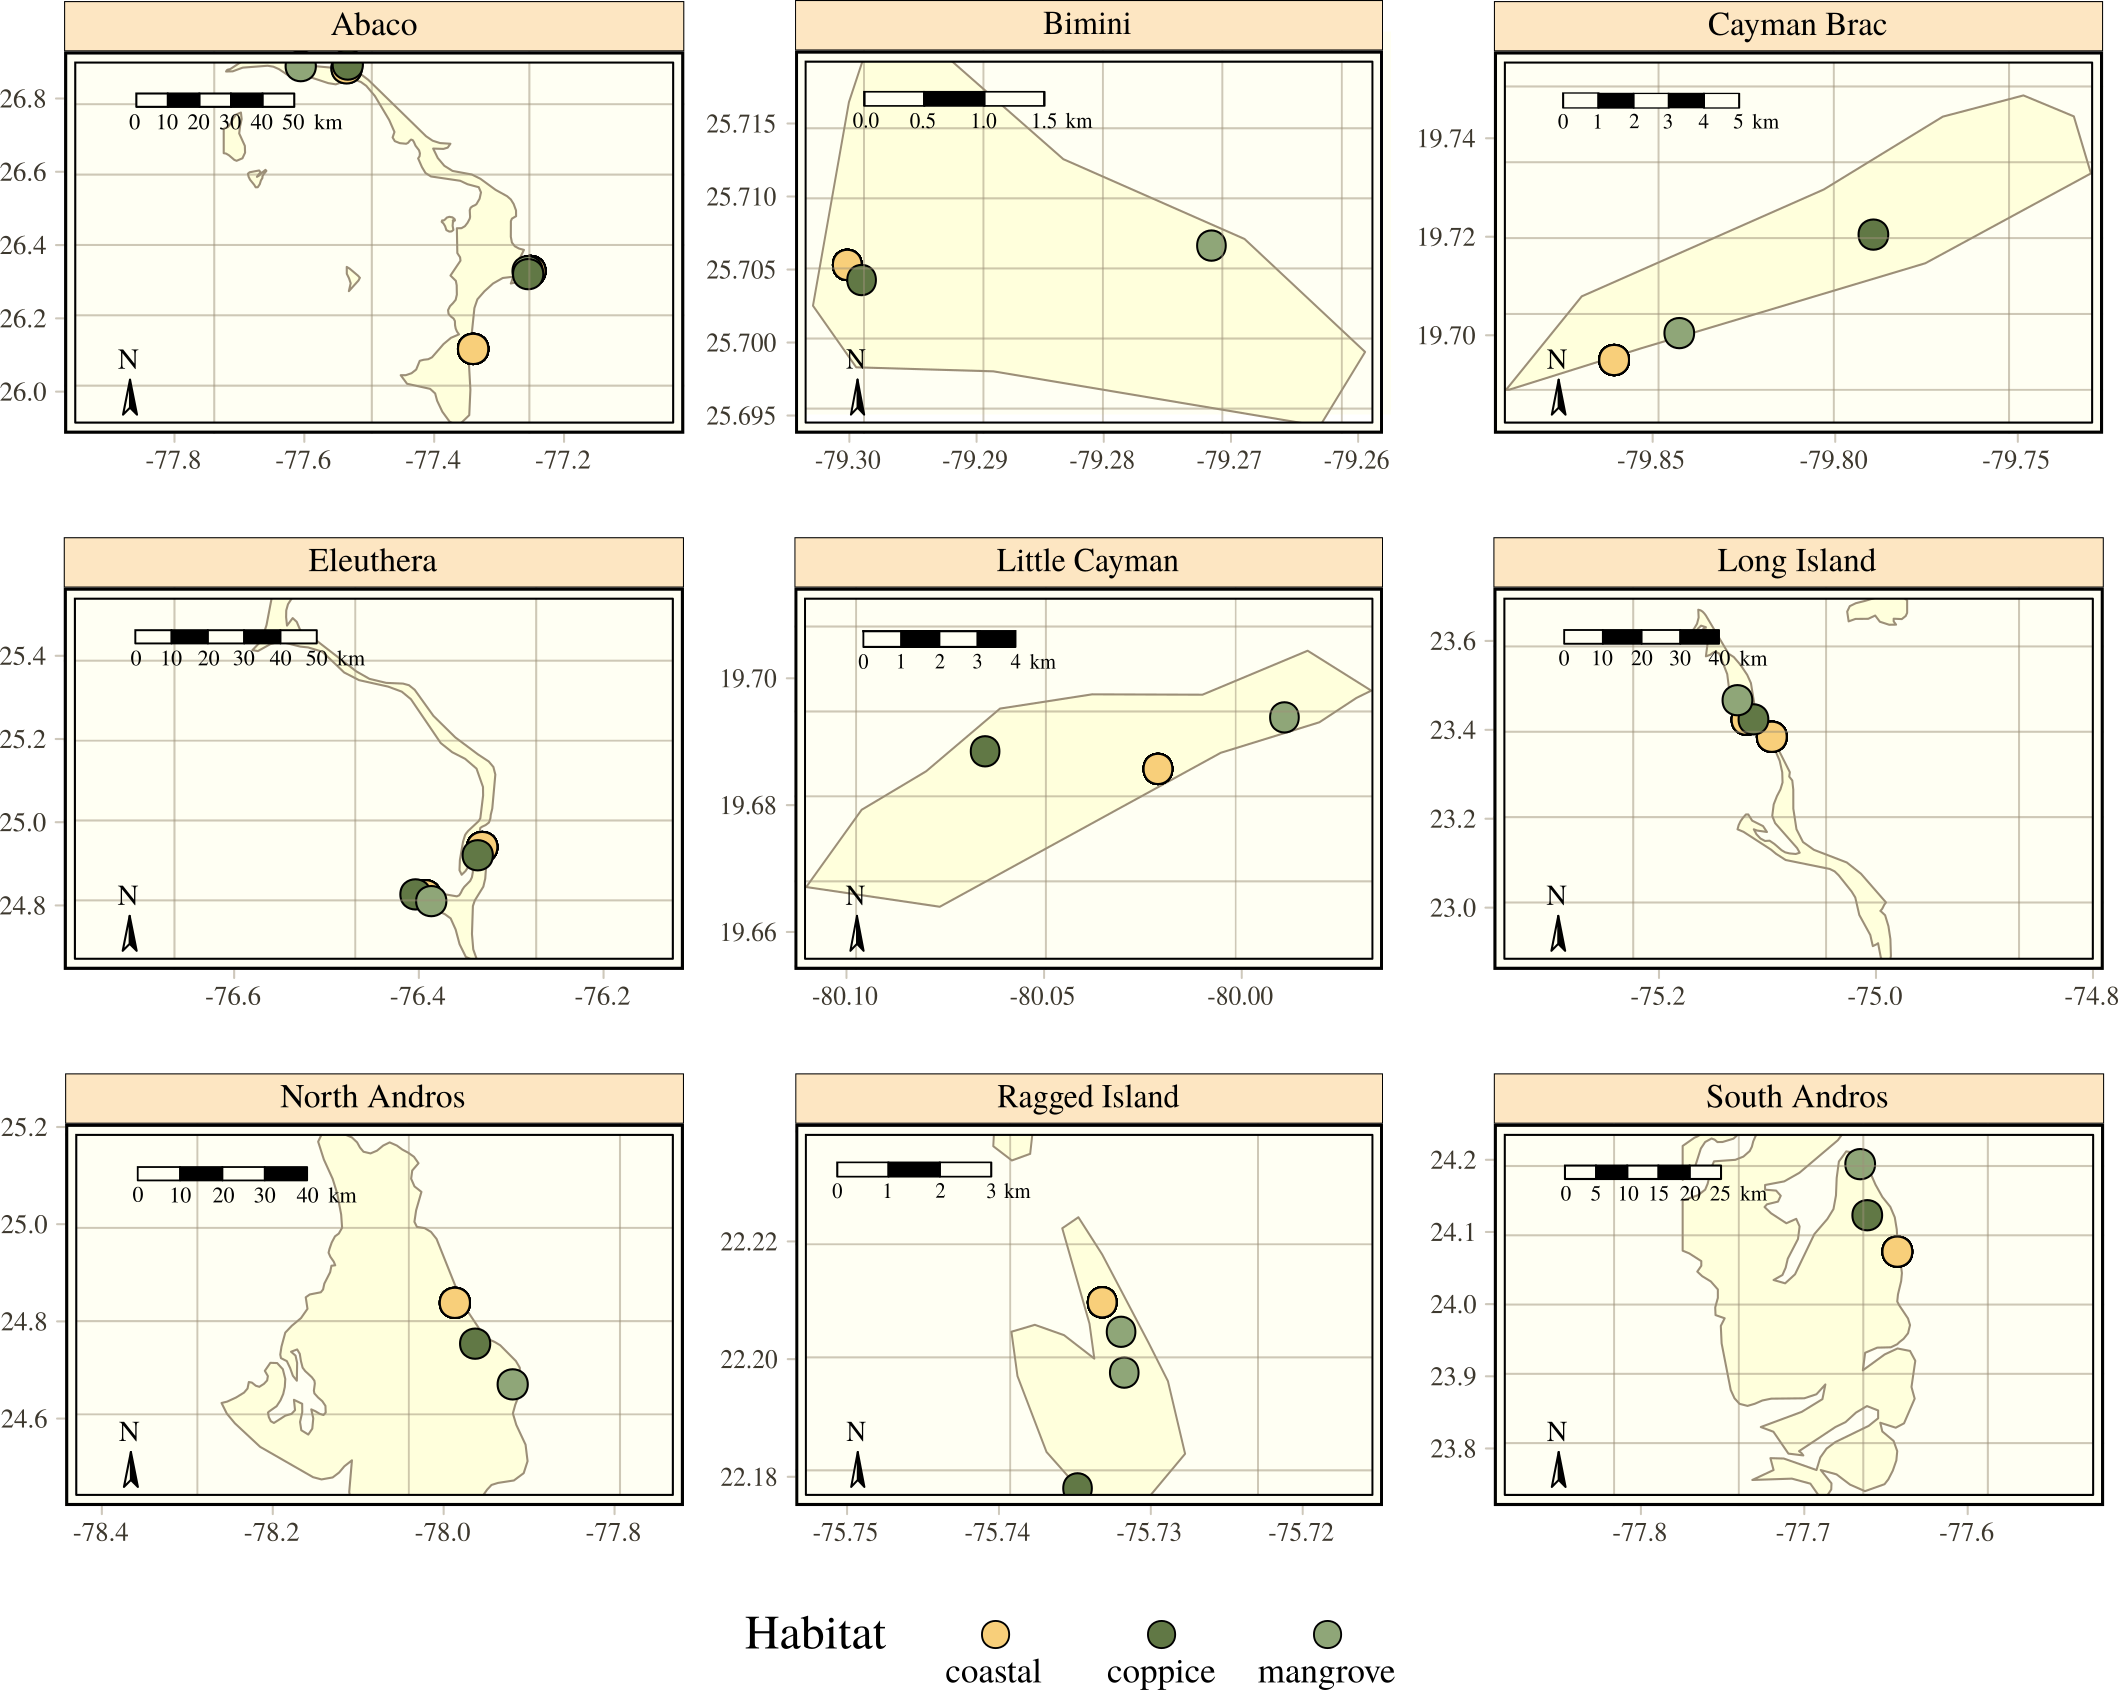
\includegraphics[width=\textwidth]{figures/island_maps.png}
	\caption{Maps of the islands. (A) Map of the West Indies with sampled islands highlighted in black. (B) Sampling sites within islands colored after their respective habitat types.}
	\label{fig:maps}
\end{figure}

\pagebreak

\begin{figure}[H]
	\centering
	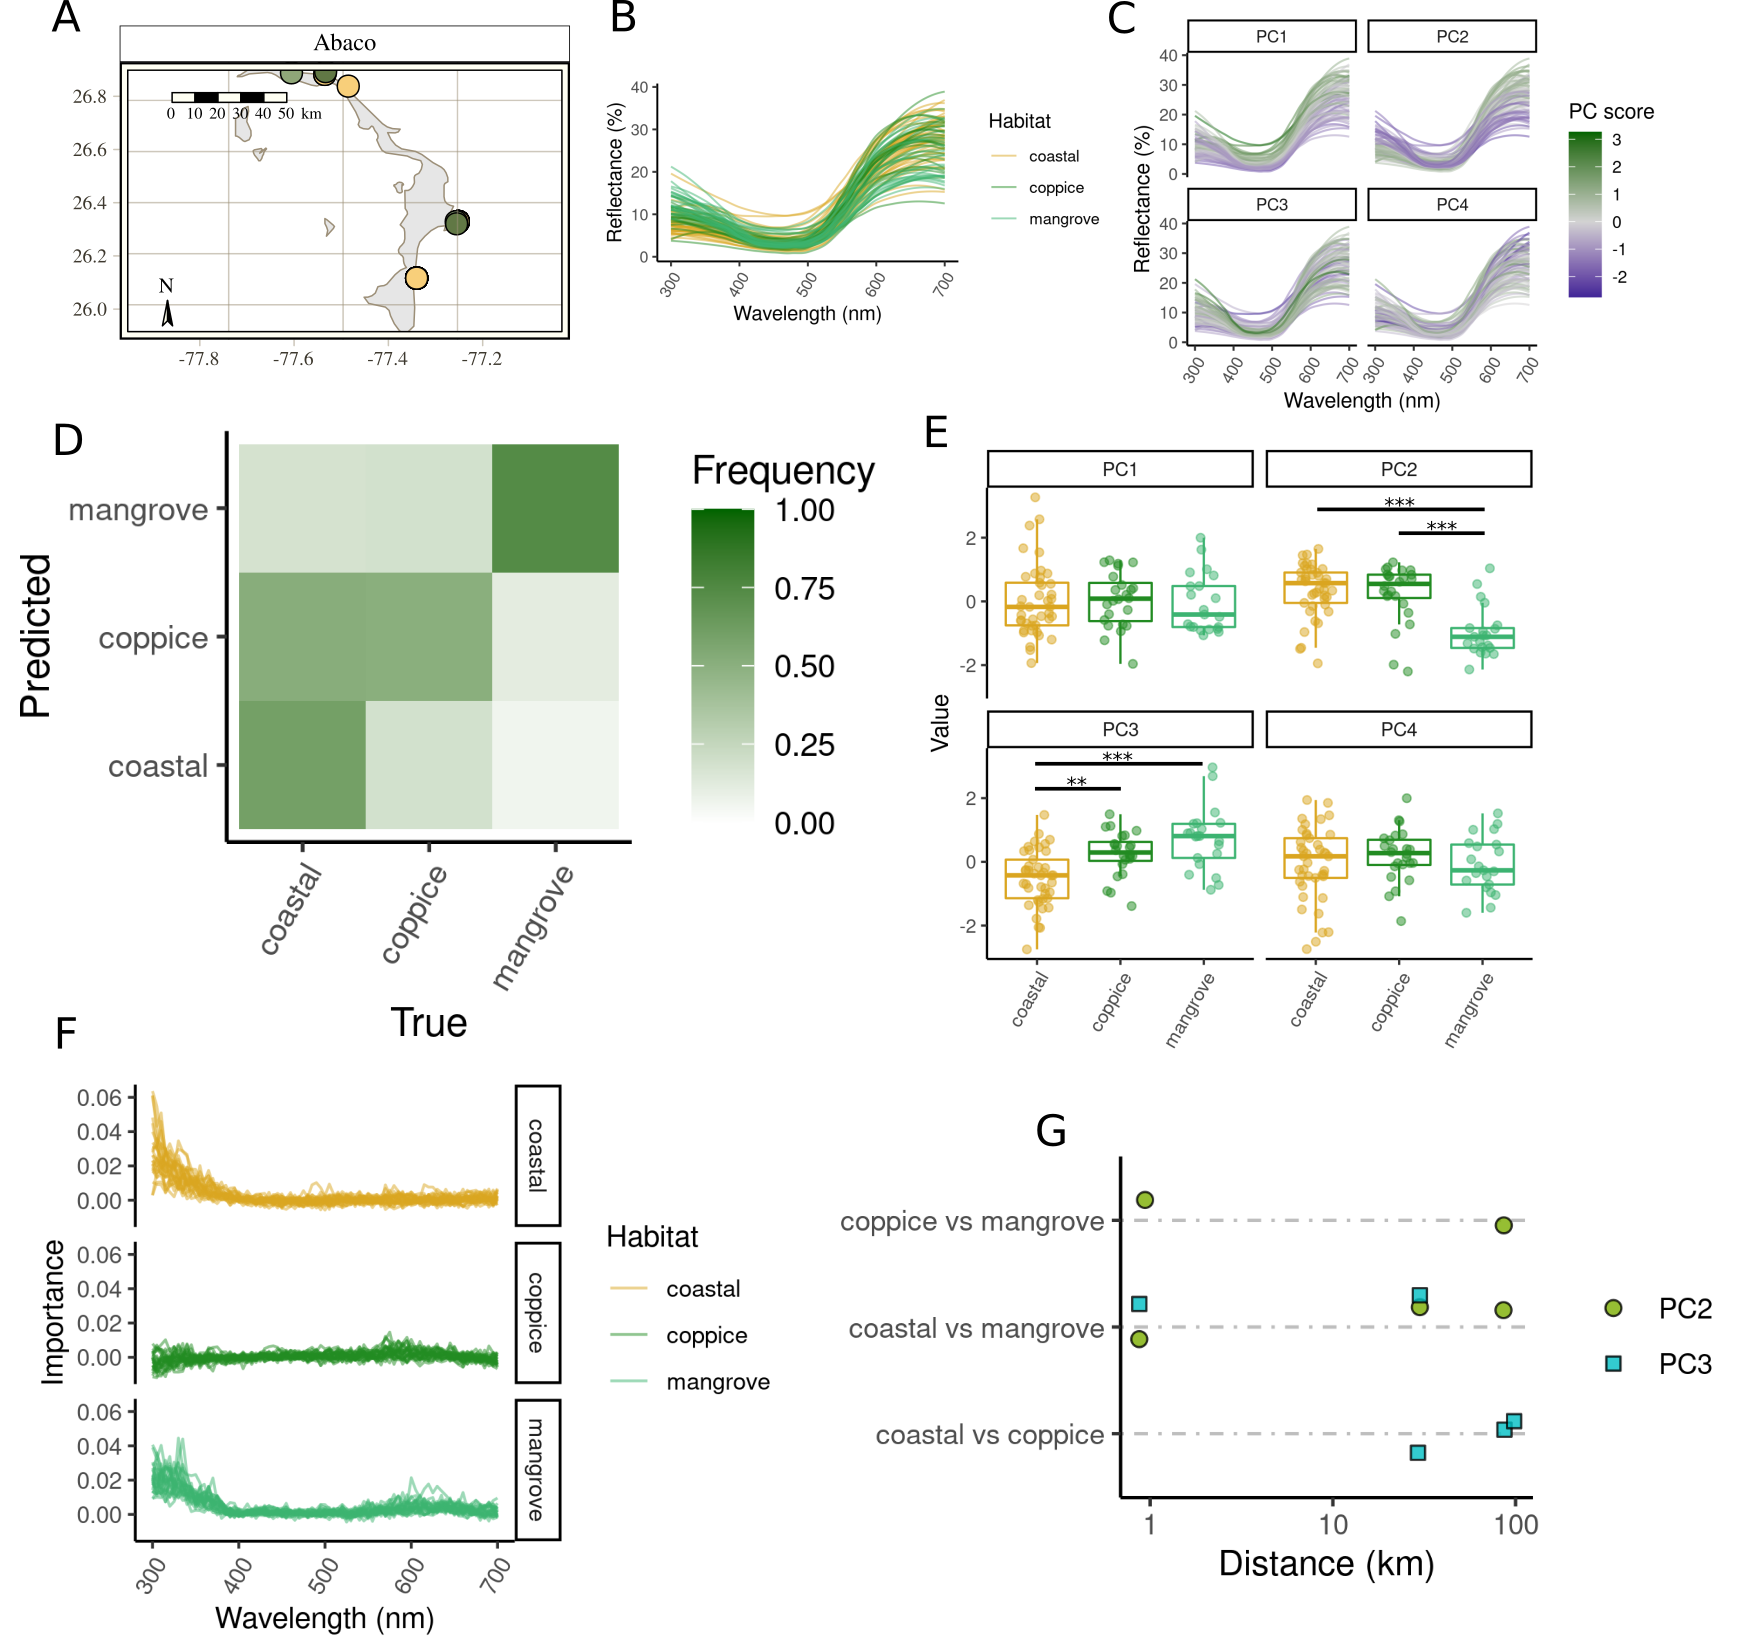
\includegraphics[width=\textwidth]{figures/Abaco_supplement.png}
	\caption{Comparison of dewlap coloration across habitats on Abaco, with extended results. (A--E) Legend as per Figure \ref{fig:Abaco}. (F) One-dimensional sensitivity analysis showing the relative importance (mean decrease in accuracy) of the various wavelengths in random forest classification of the whole spectrum. (G) Geographical distance between sites where significant differences were detected in within-island principal component scores (Wilcoxon test, Benjamini-Hochberg correction, $P < 0.05$), including only pairs of sites whose habitats were involved in between-habitat dewlap differences.}
	\label{fig:Abaco_supplement}
\end{figure}

\pagebreak

\begin{figure}[H]
	\centering
	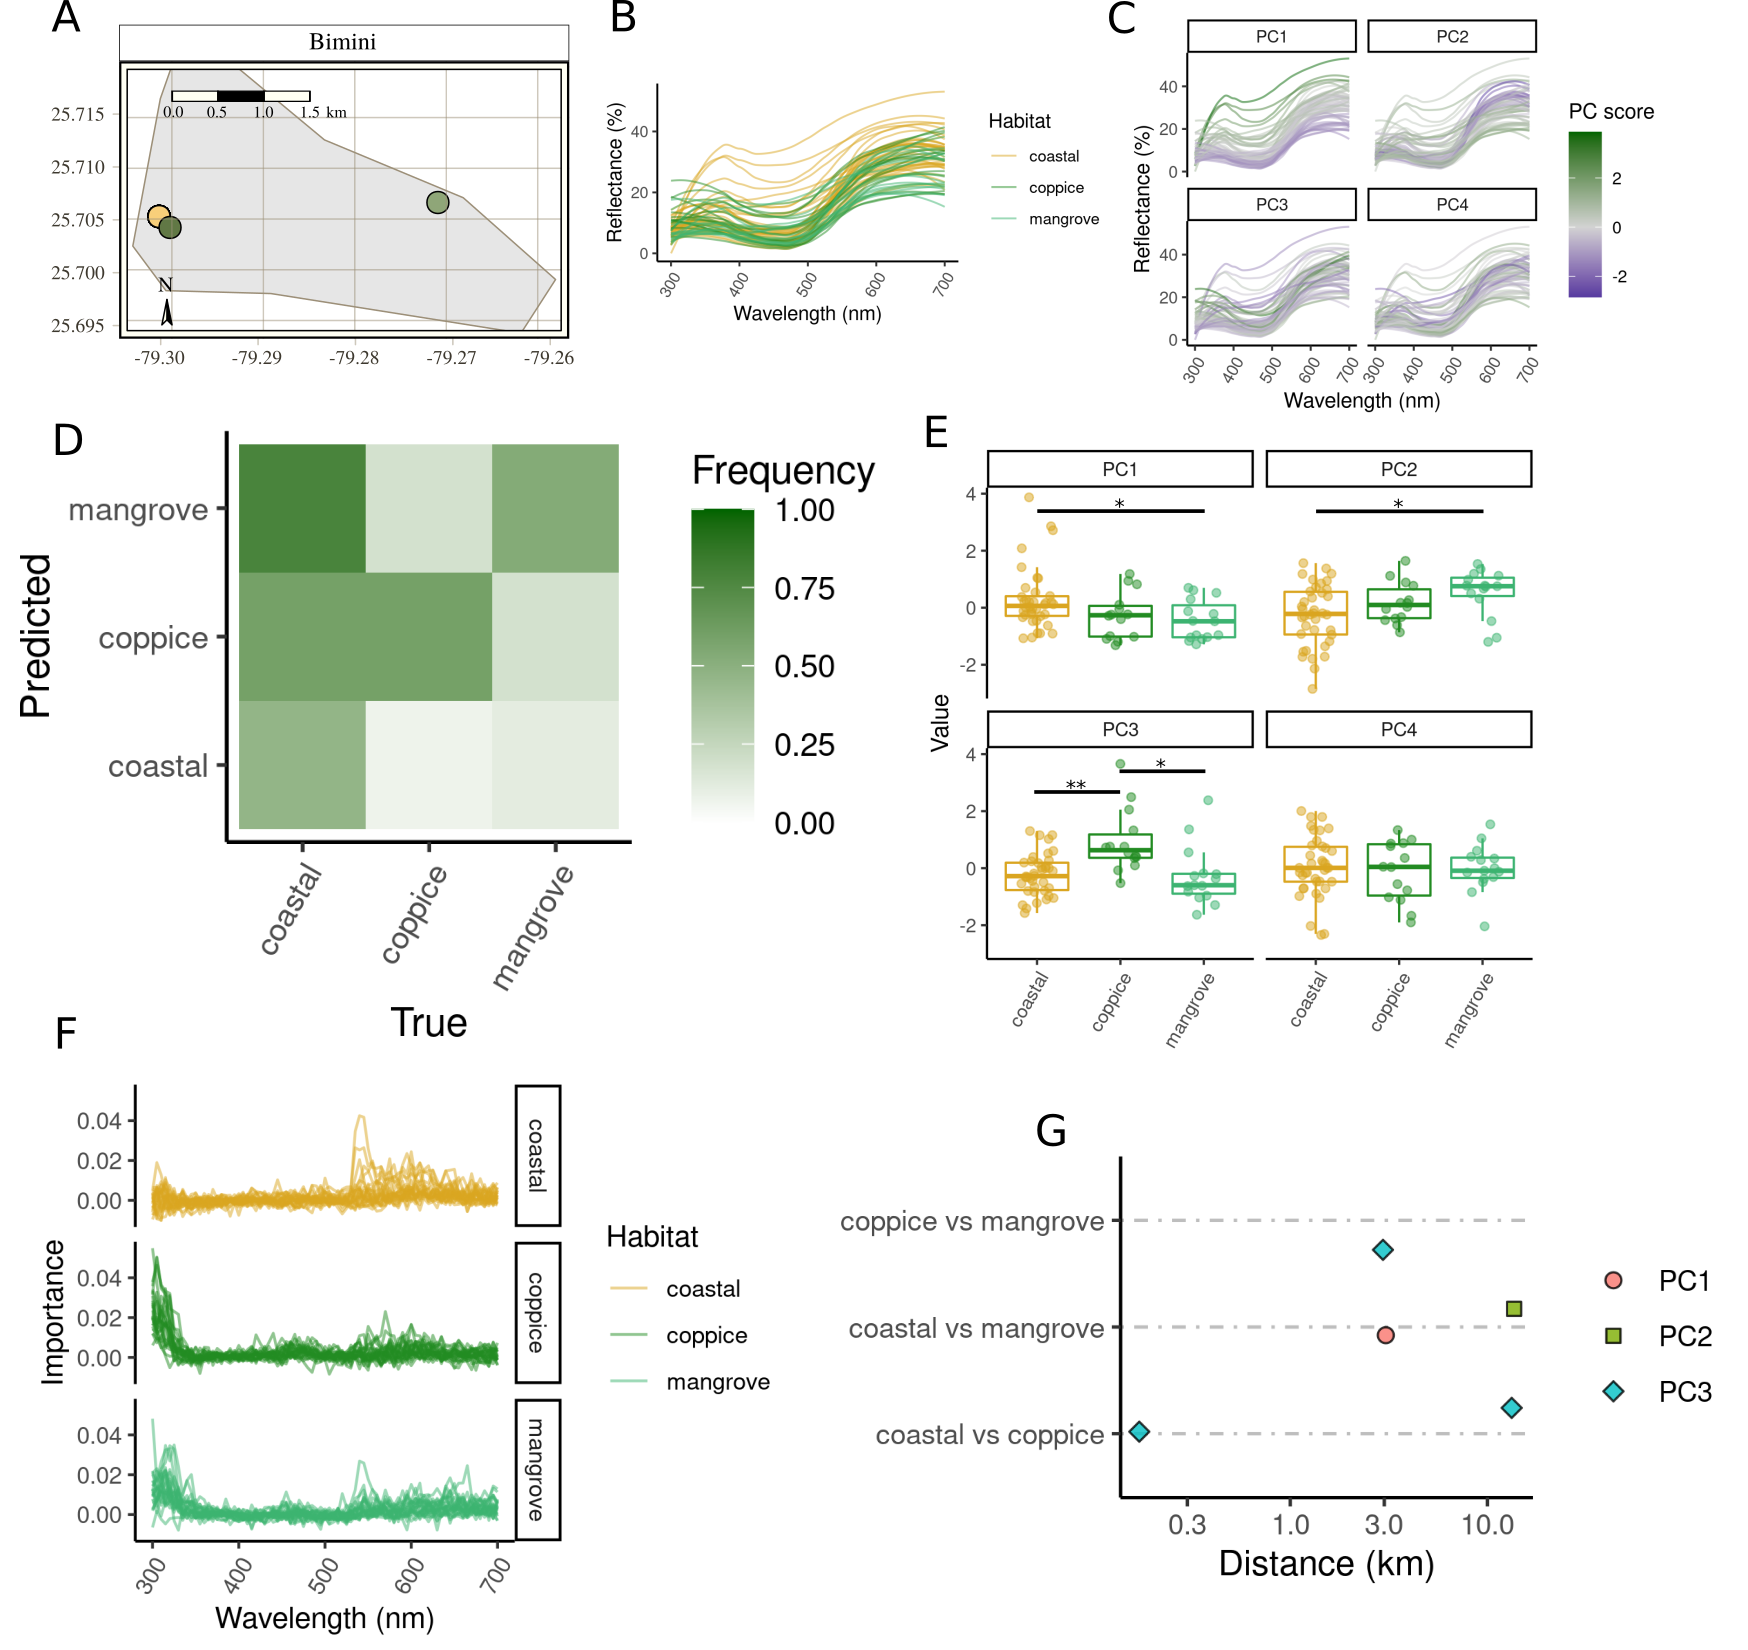
\includegraphics[width=\textwidth]{figures/Bimini_supplement.png}
	\caption{Comparison of dewlap coloration across habitats on Bimini. Legend is as per Figure \ref{fig:Abaco_supplement}.}
	\label{fig:Bimini}
\end{figure}

\pagebreak

\begin{figure}[H]
	\centering
	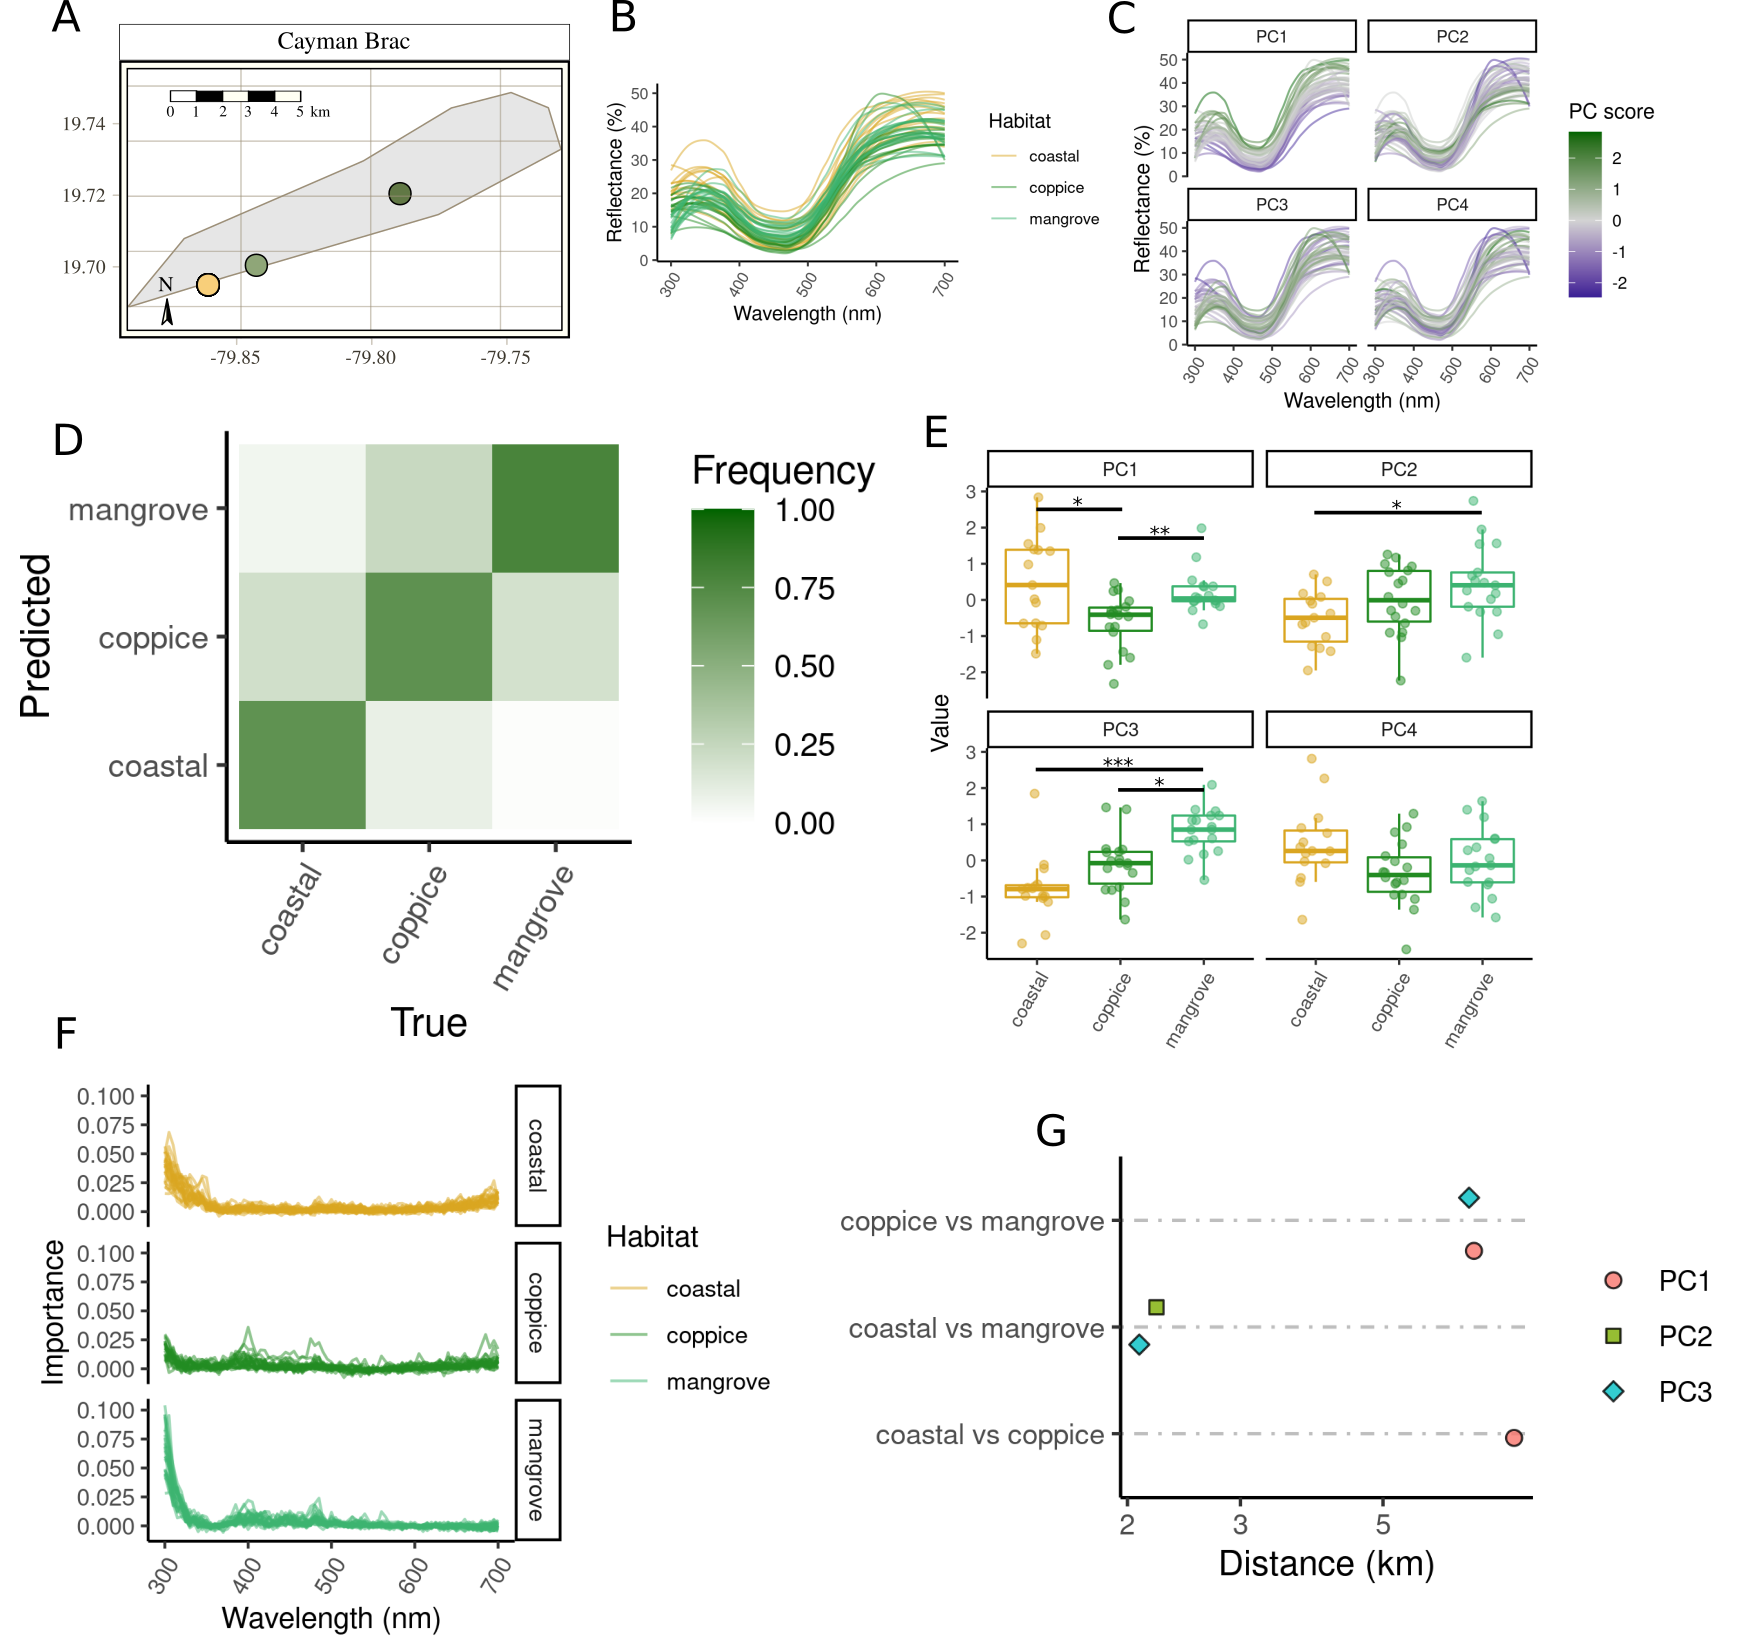
\includegraphics[width=\textwidth]{figures/CaymanBrac_supplement.png}
	\caption{Comparison of dewlap coloration across habitats on Cayman Brac. Legend is as per Figure \ref{fig:Abaco_supplement}.}
	\label{fig:CaymanBrac}
\end{figure}

\pagebreak

\begin{figure}[H]
	\centering
	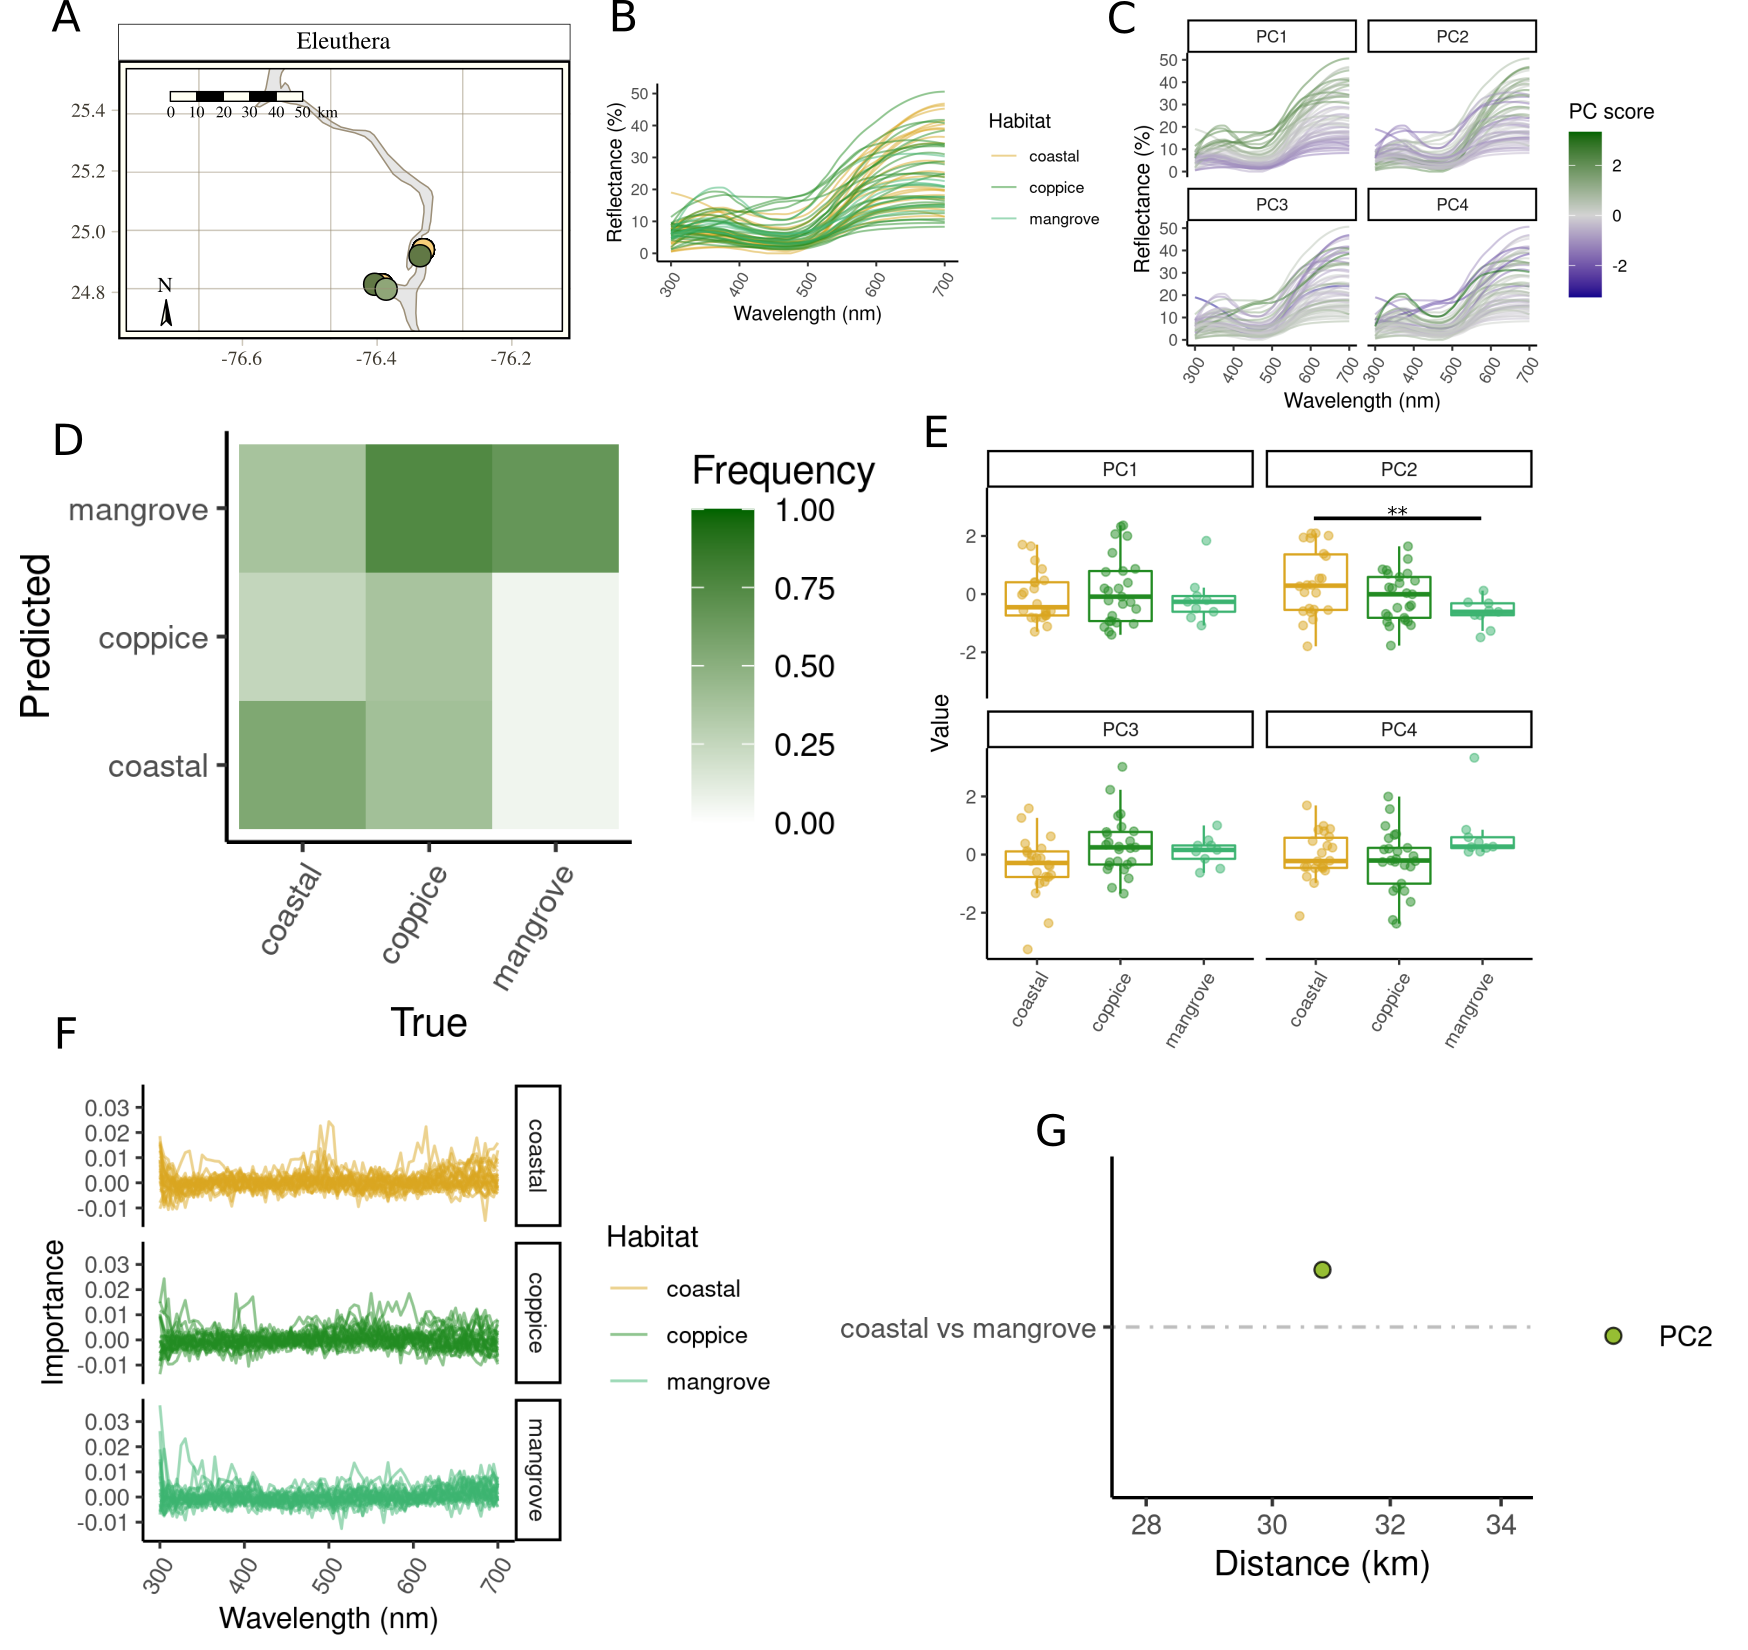
\includegraphics[width=\textwidth]{figures/Eleuthera_supplement.png}
	\caption{Comparison of dewlap coloration across habitats on Eleuthera. Legend is as per Figure \ref{fig:Abaco_supplement}.}
	\label{fig:Eleuthera}
\end{figure}

\pagebreak

\begin{figure}[H]
	\centering
	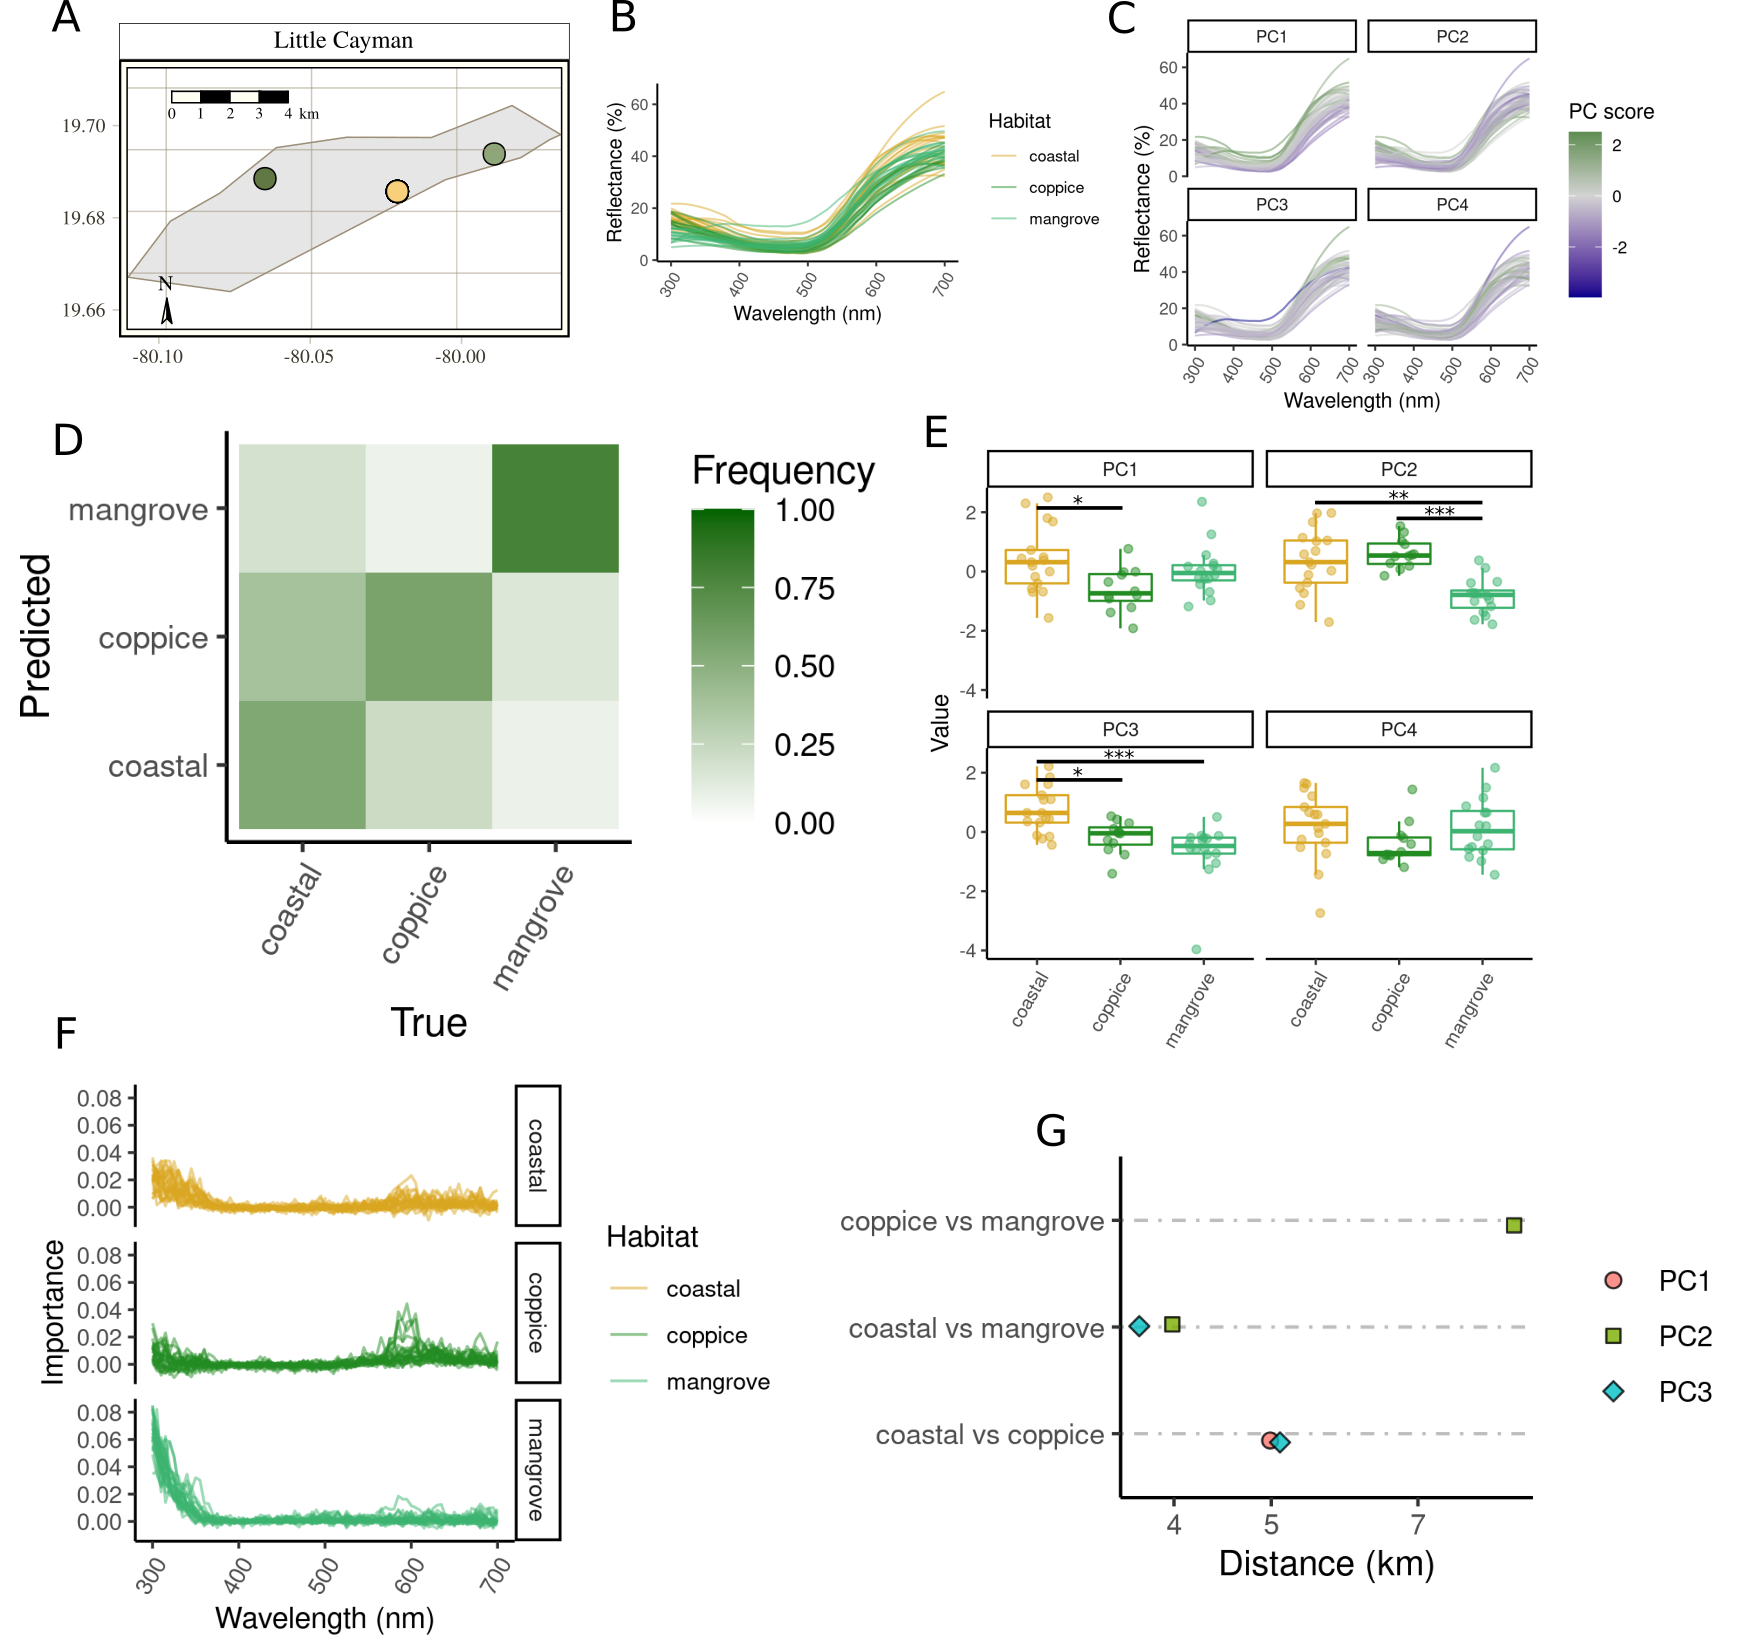
\includegraphics[width=\textwidth]{figures/LittleCayman_supplement.png}
	\caption{Comparison of dewlap coloration across habitats on Little Cayman. Legend is as per Figure \ref{fig:Abaco_supplement}.}
	\label{fig:LittleCayman}
\end{figure}

\pagebreak

\begin{figure}[H]
	\centering
	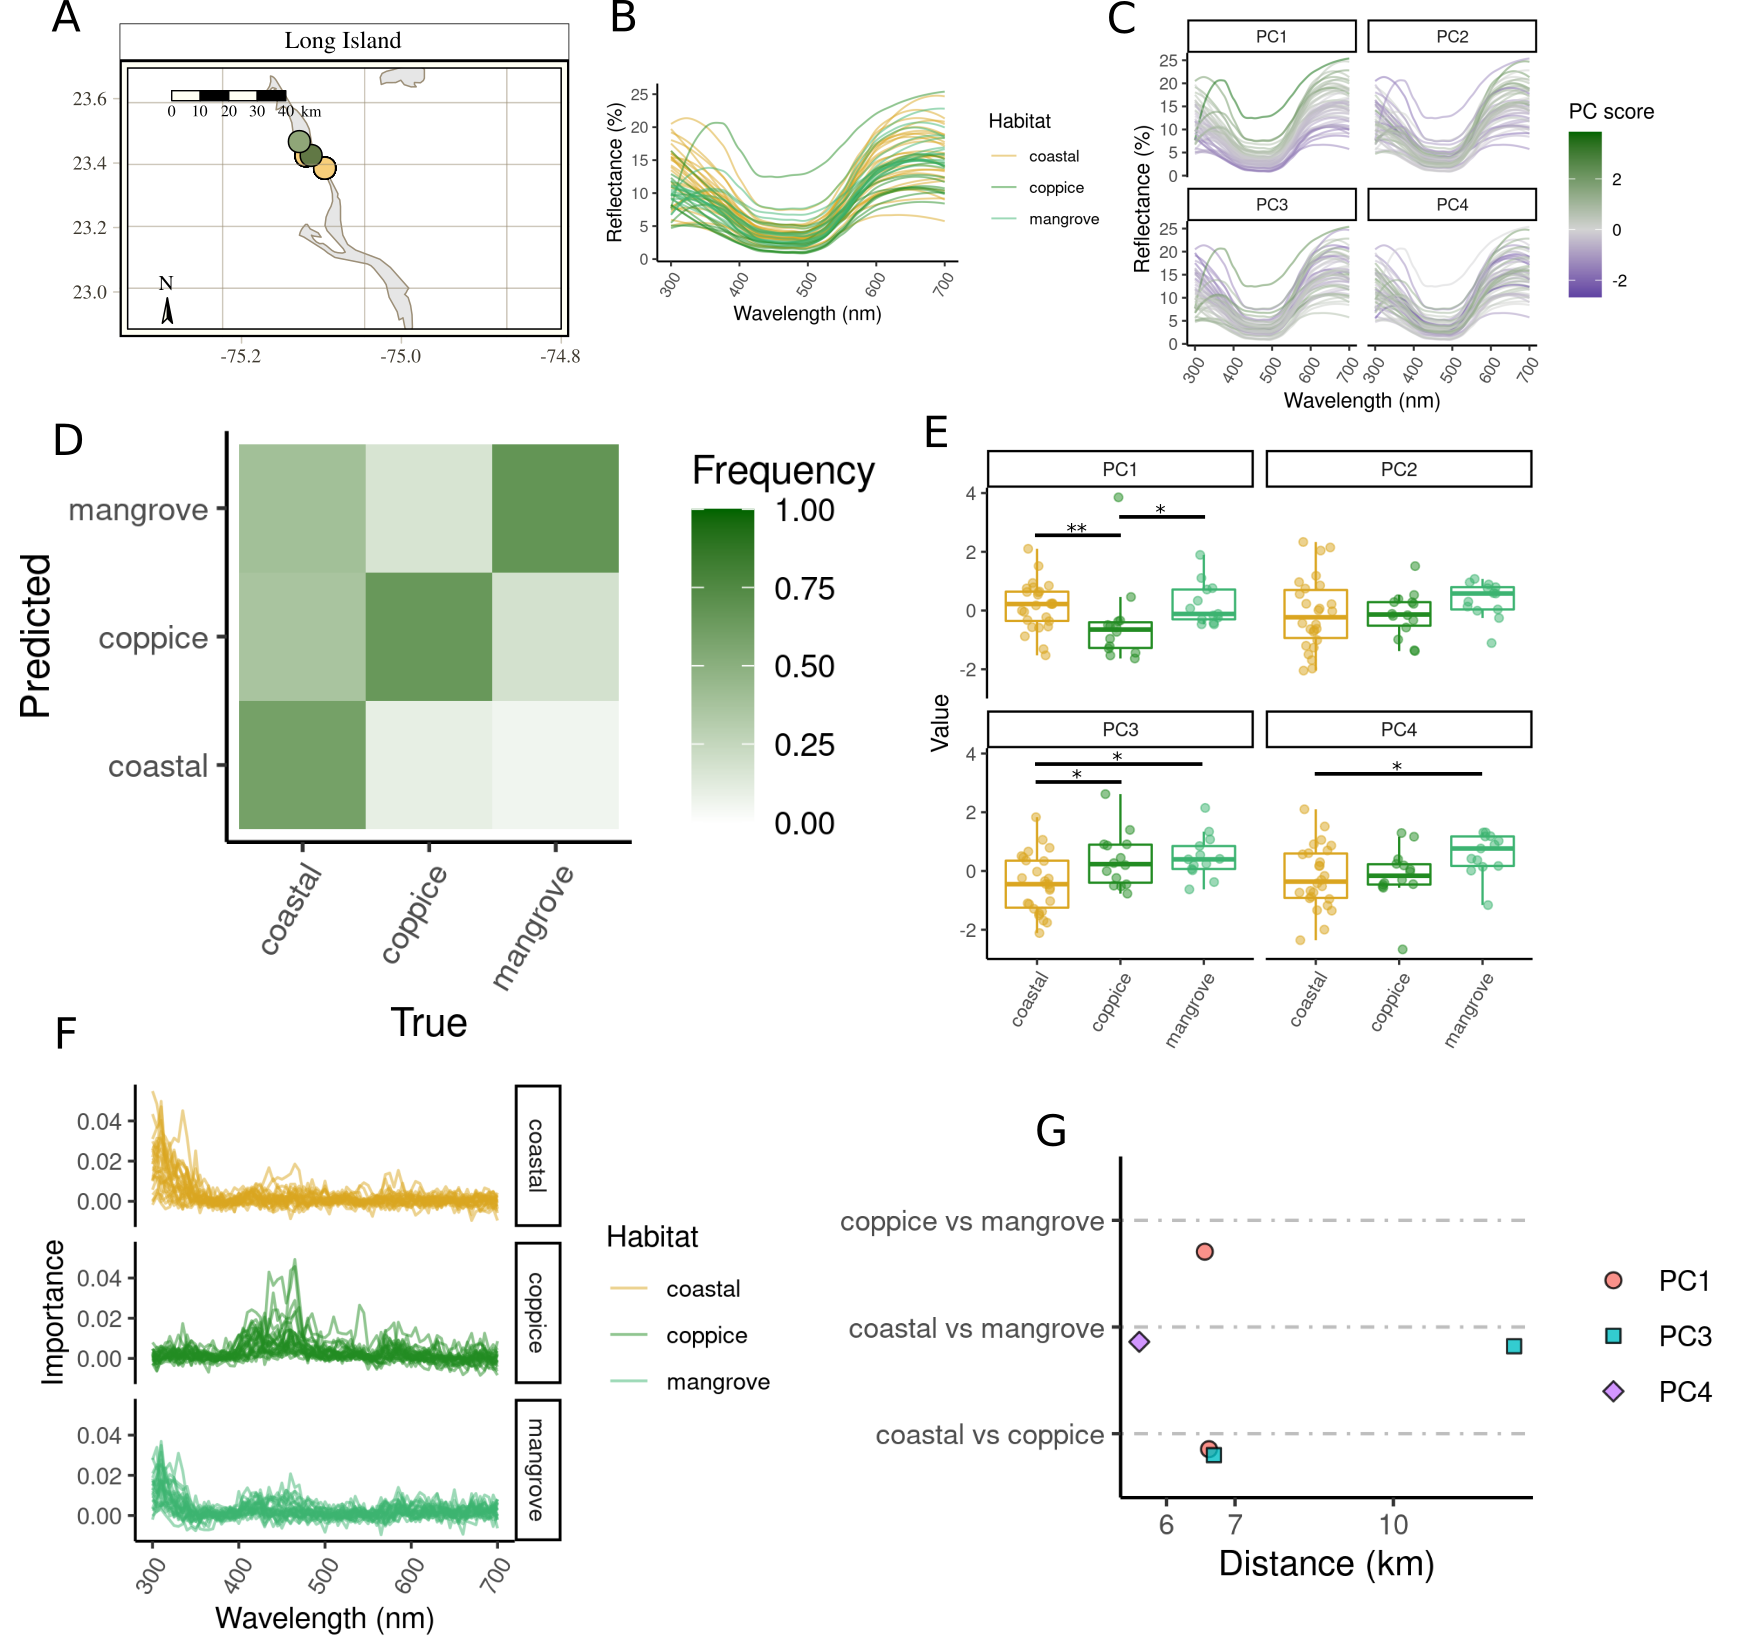
\includegraphics[width=\textwidth]{figures/LongIsland_supplement.png}
	\caption{Comparison of dewlap coloration across habitats on Long Island. Legend is as per Figure \ref{fig:Abaco_supplement}.}
	\label{fig:LongIsland}
\end{figure}

\pagebreak

\begin{figure}[H]
	\centering
	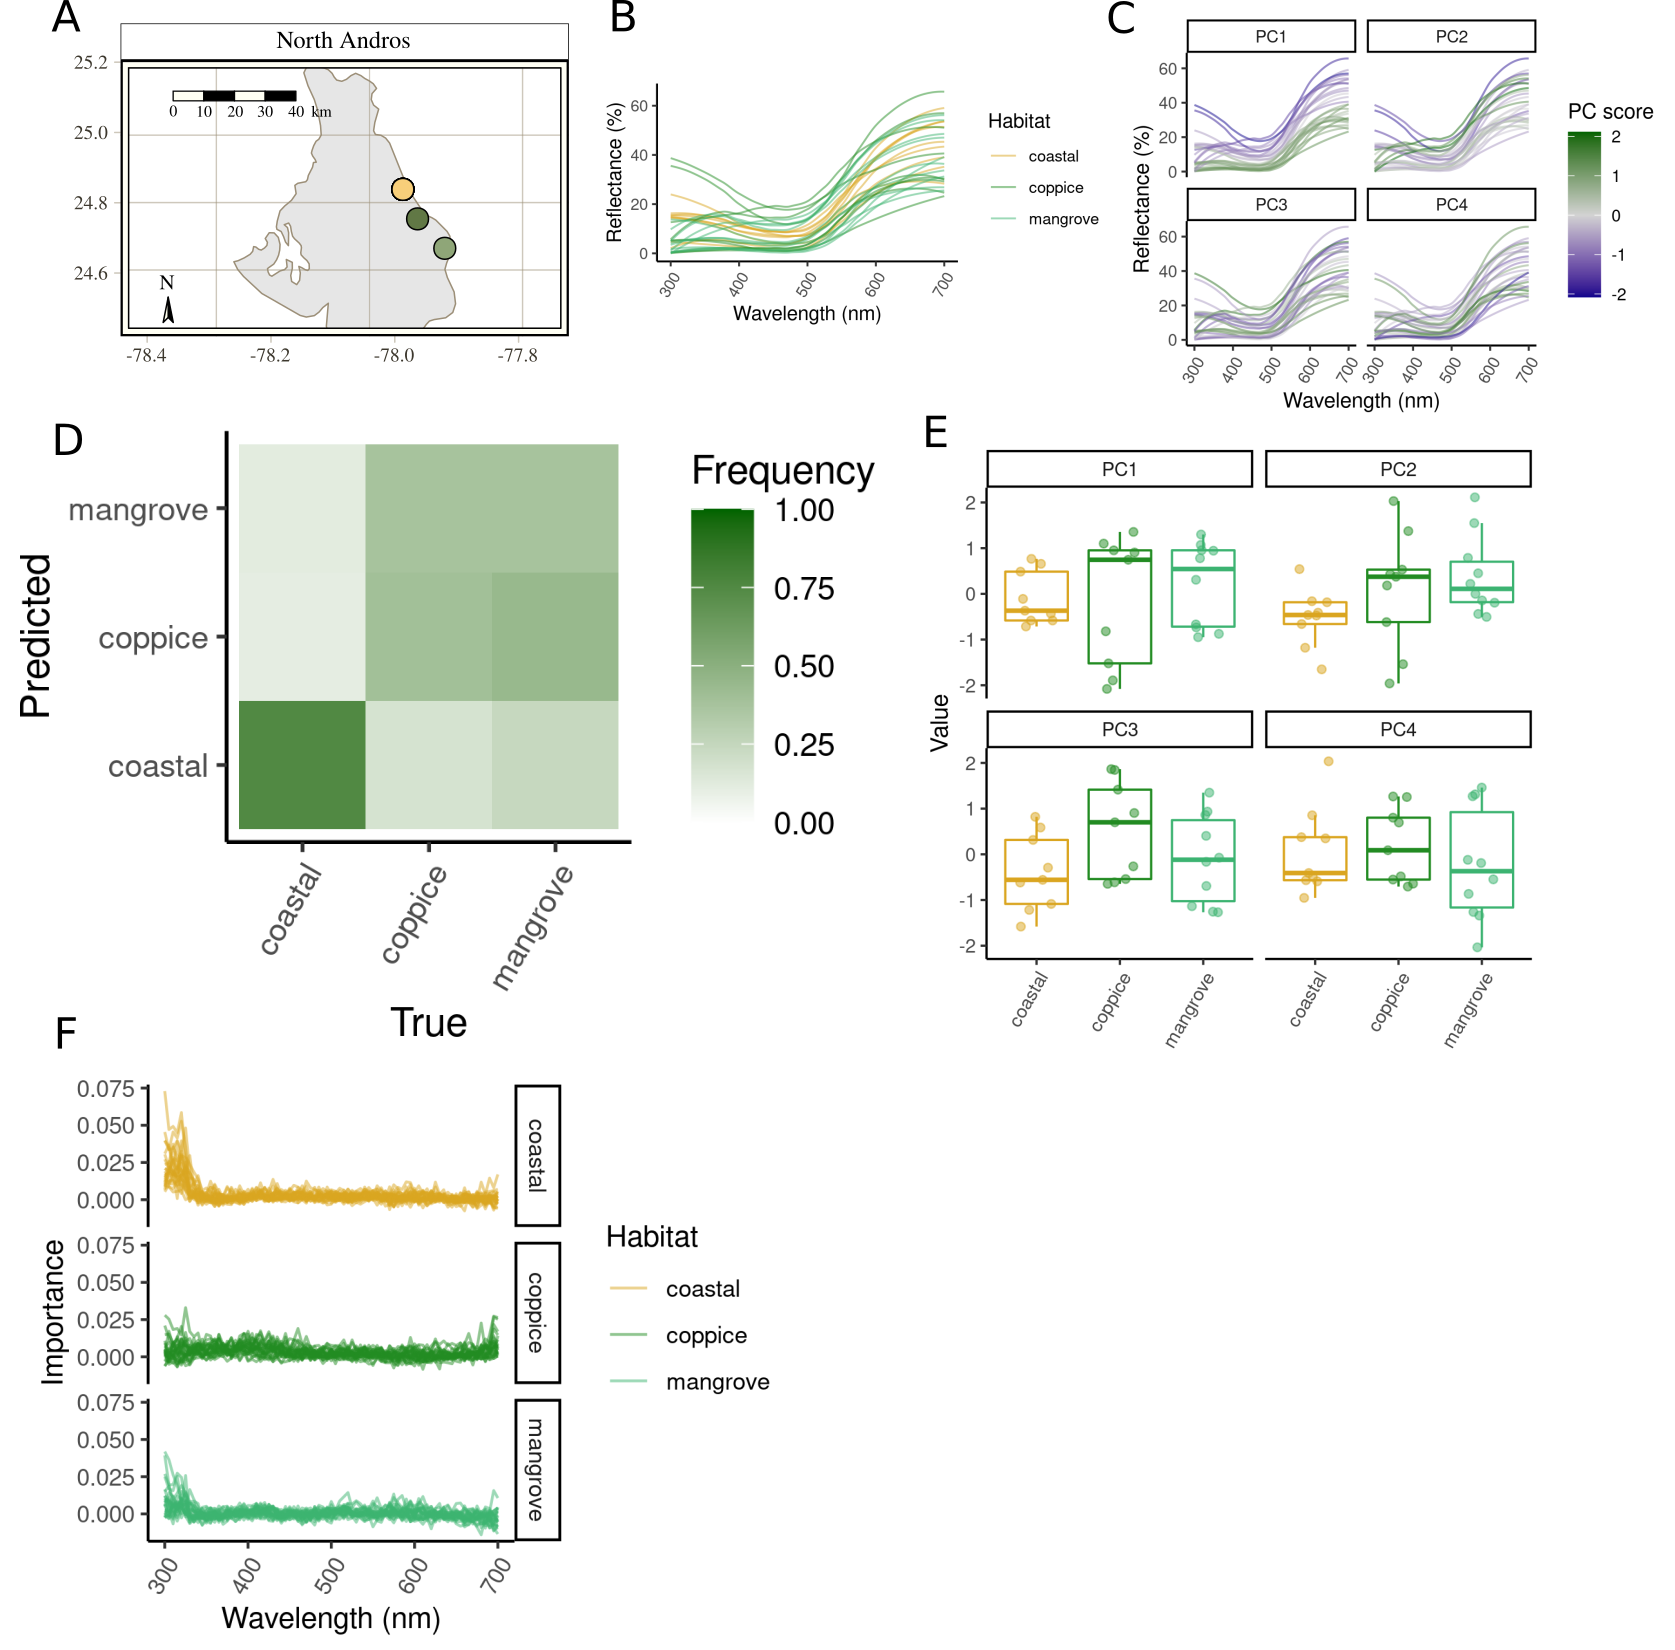
\includegraphics[width=\textwidth]{figures/NorthAndros_supplement.png}
	\caption{Comparison of dewlap coloration across habitats on North Andros. Legend is as per Figure \ref{fig:Abaco_supplement}\sout{, but without panel G}.}
	\label{fig:NorthAndros}
\end{figure}

\pagebreak

\begin{figure}[H]
	\centering
	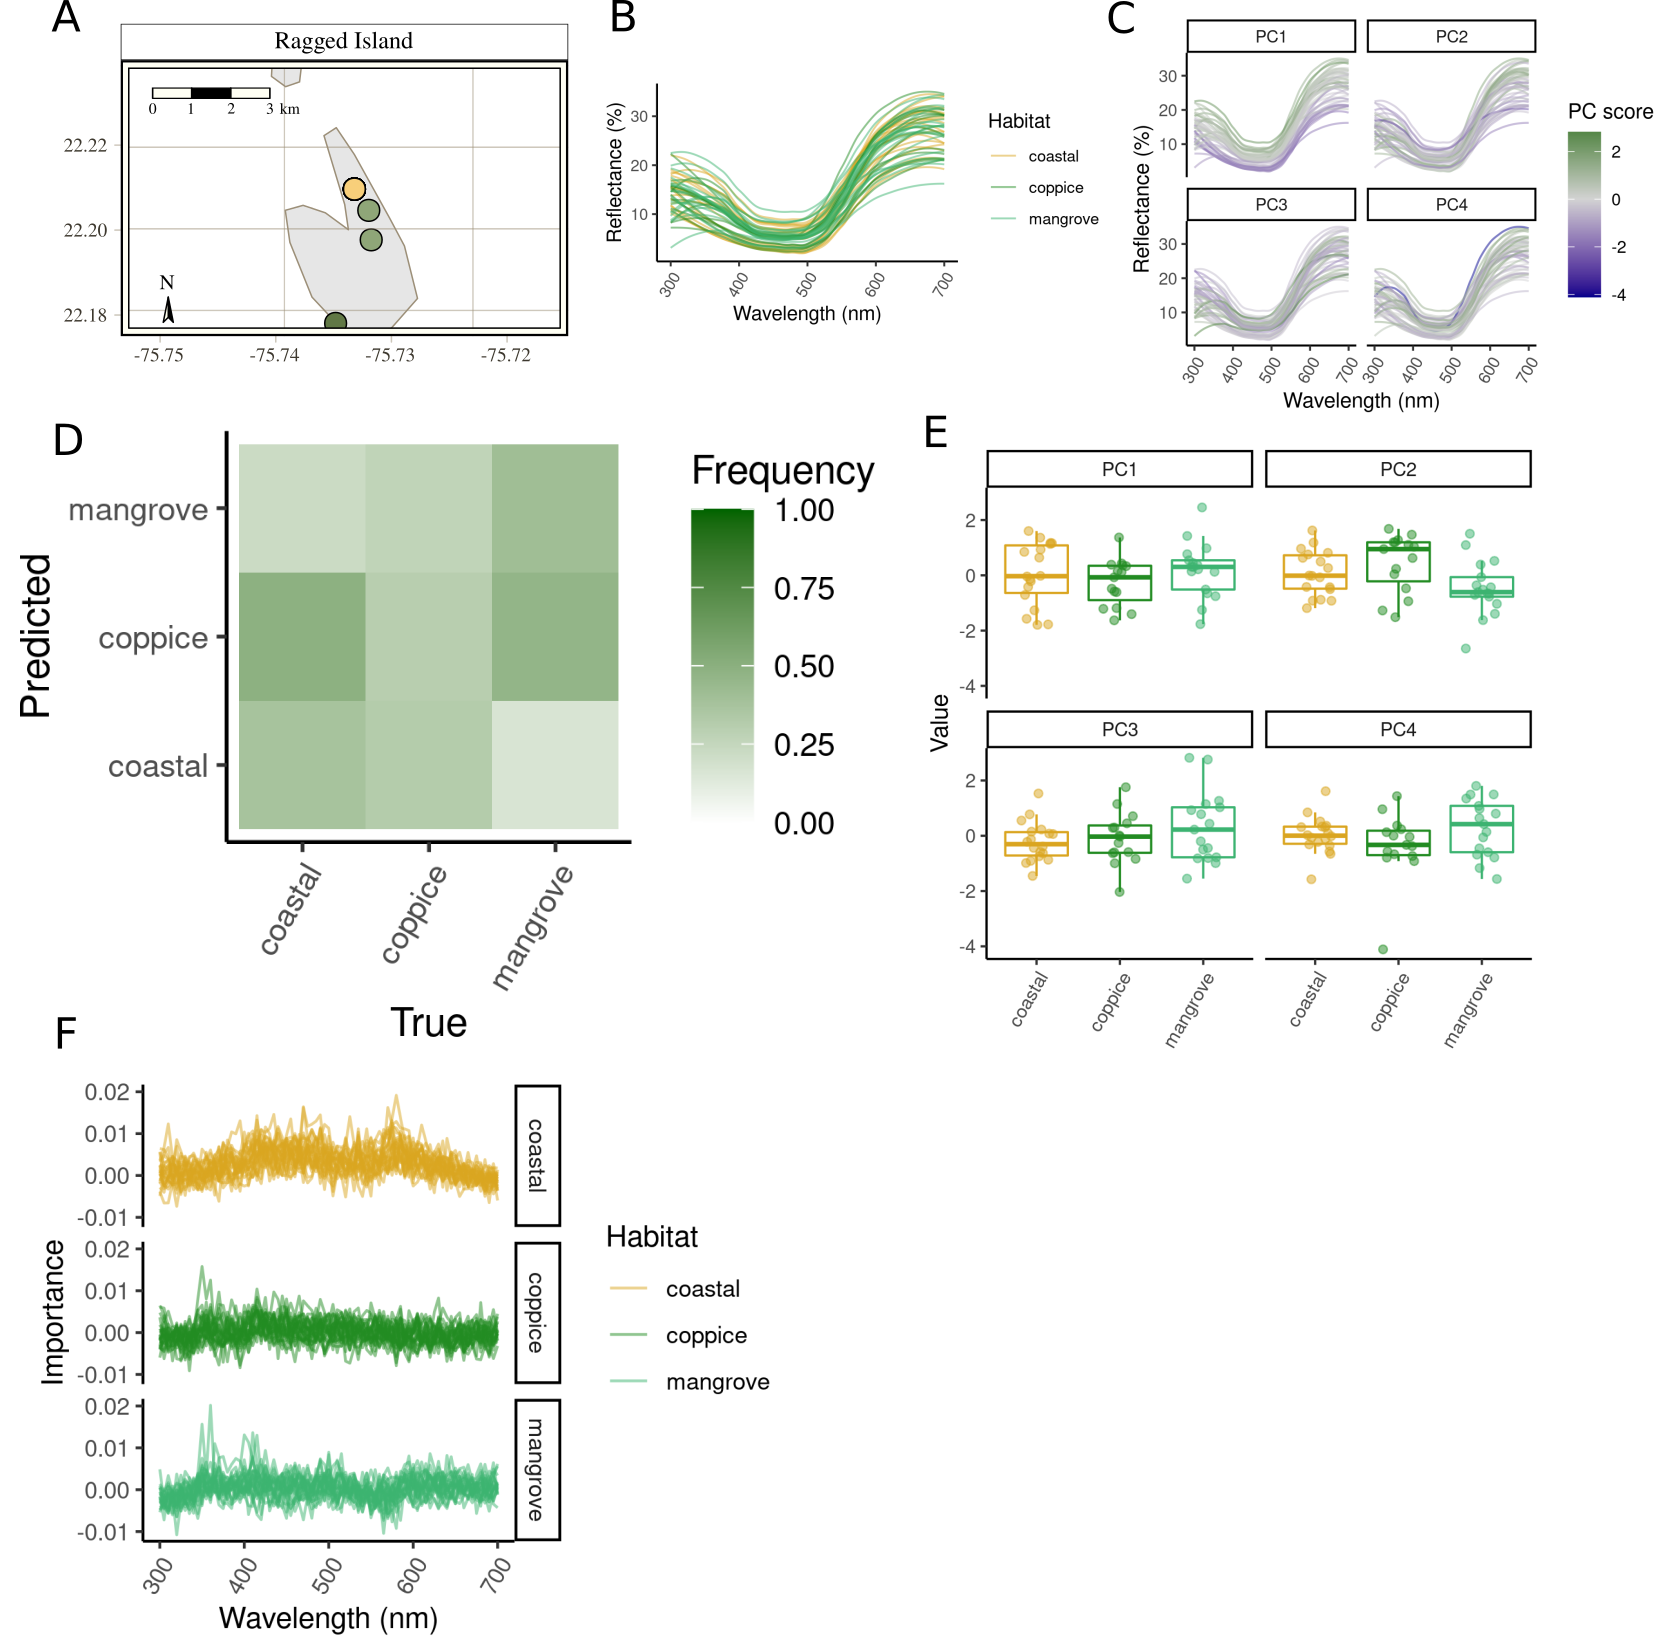
\includegraphics[width=\textwidth]{figures/RaggedIsland_supplement.png}
	\caption{Comparison of dewlap coloration across habitats on Ragged Island. Legend is as per Figure \ref{fig:Abaco_supplement}, but without panel G.}
	\label{fig:RaggedIsland}
\end{figure}

\pagebreak

\begin{figure}[H]
	\centering
	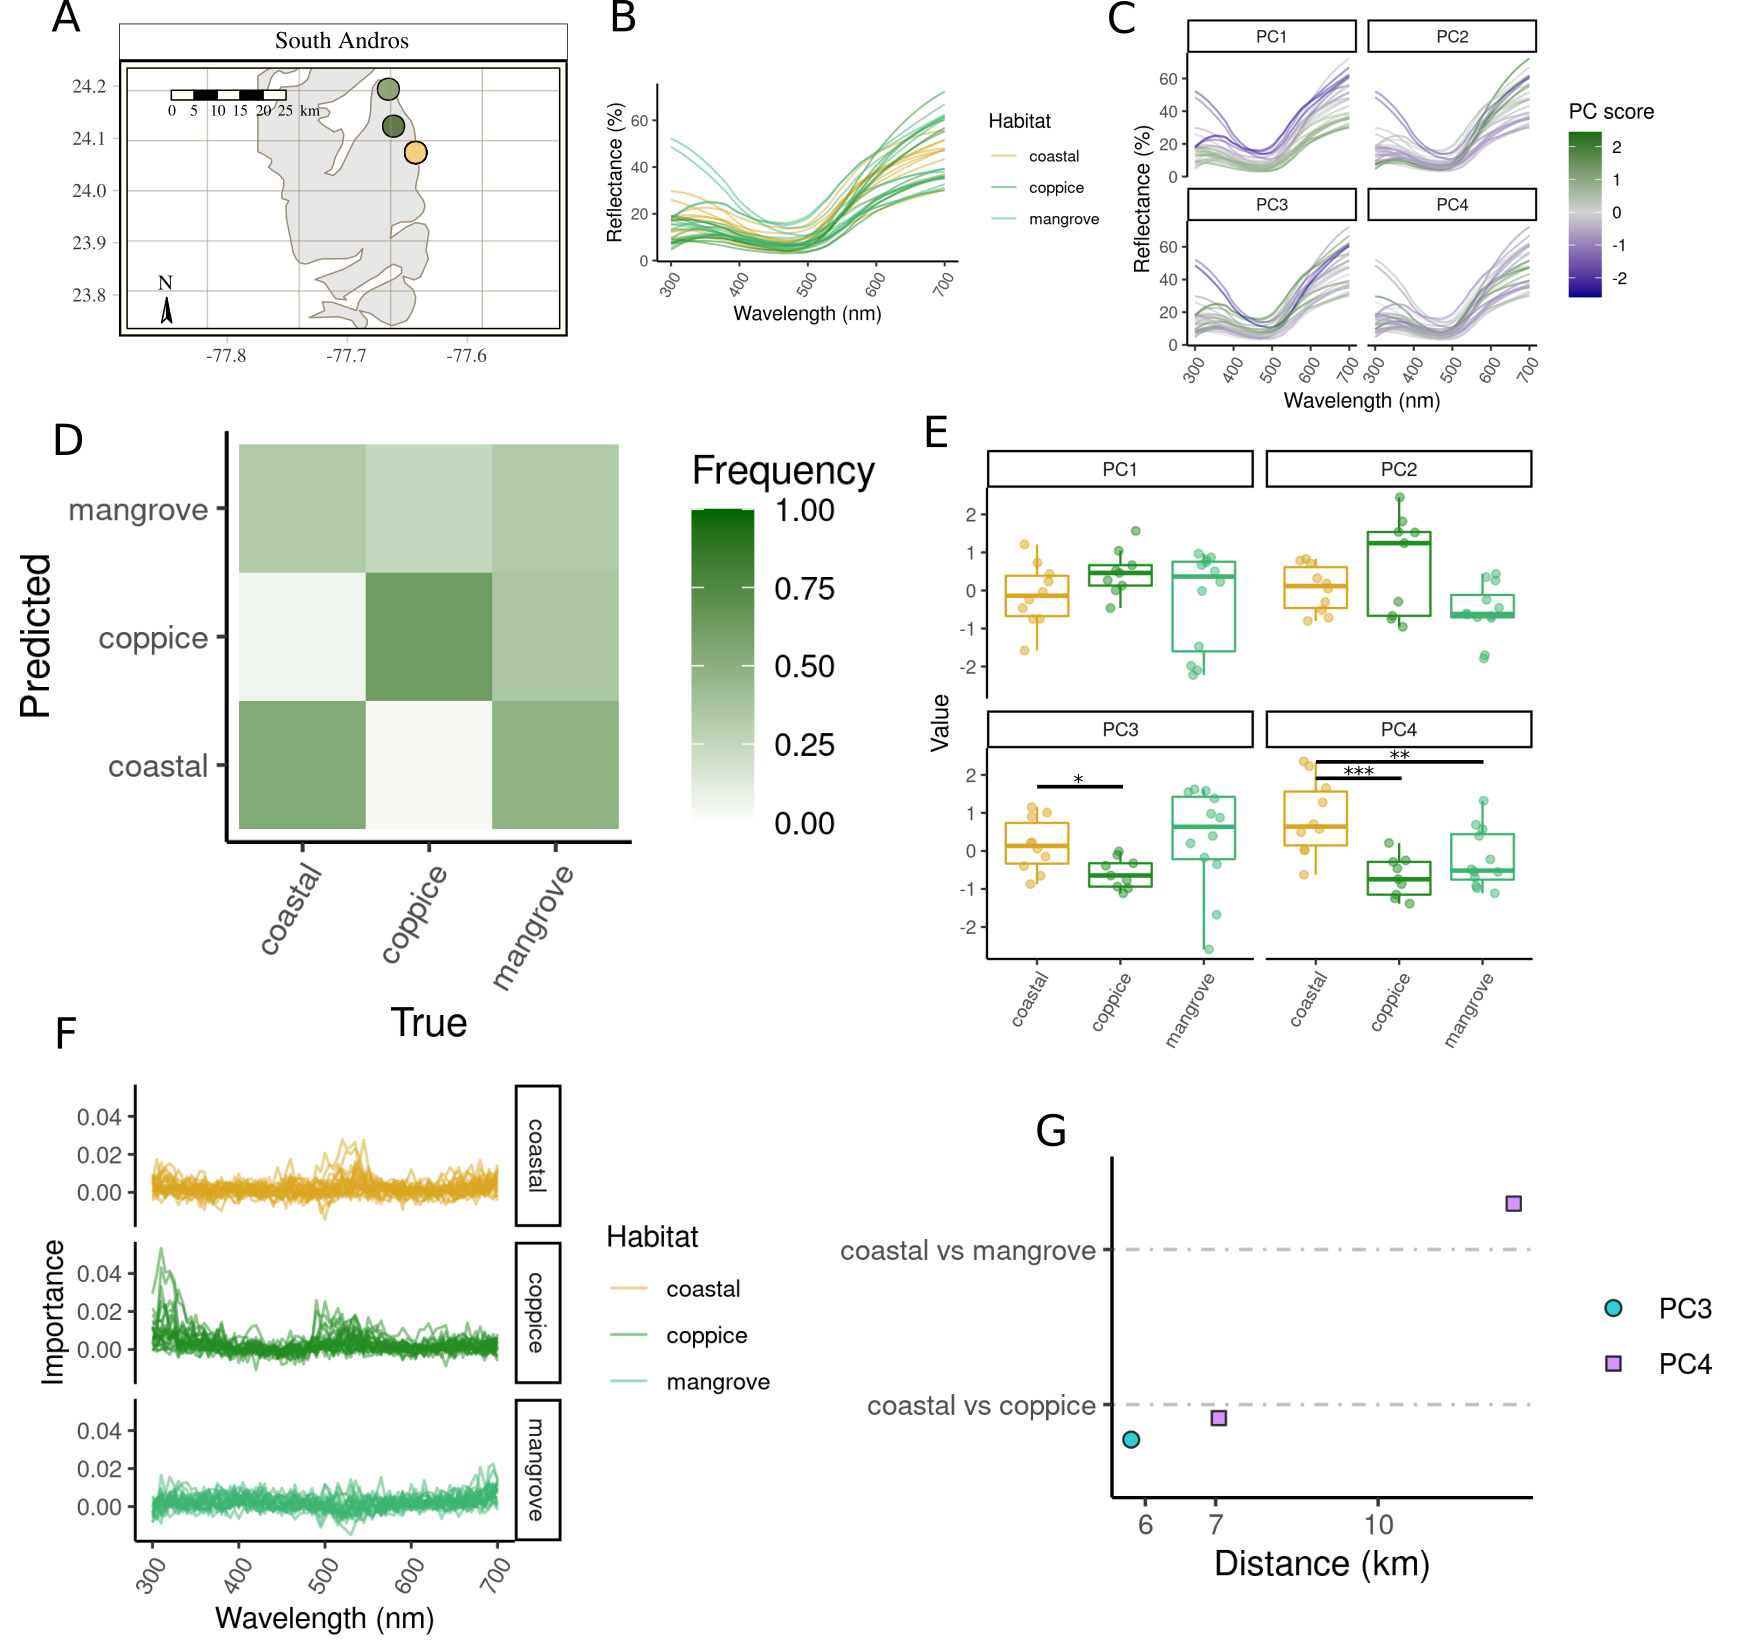
\includegraphics[width=\textwidth]{figures/SouthAndros_supplement.png}
	\caption{Comparison of dewlap coloration across habitats on South Andros. Legend is as per Figure \ref{fig:Abaco_supplement}\textcolor{olive}{, but without panel G}.}
	\label{fig:SouthAndros}
\end{figure}

\pagebreak

\begin{figure}[H]
	\centering
	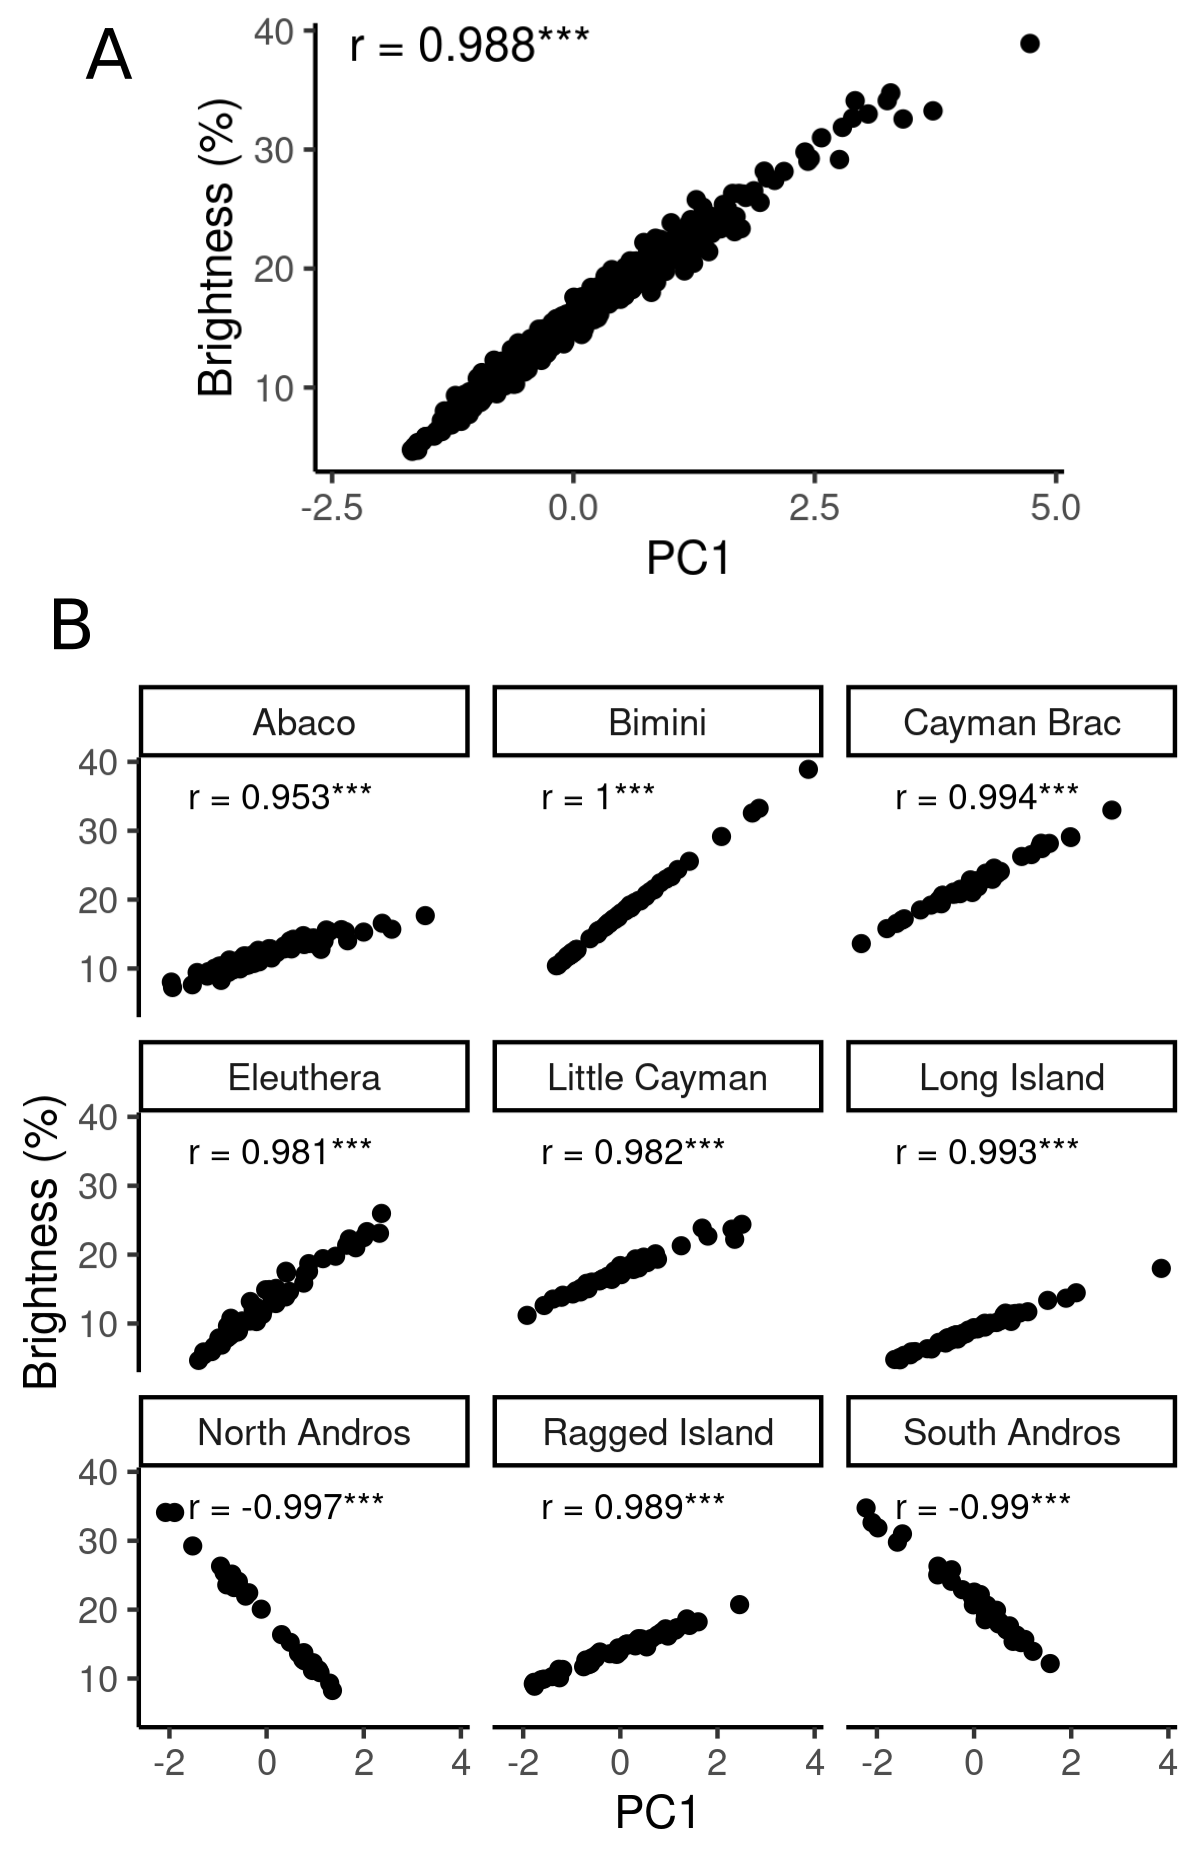
\includegraphics[width=0.8\textwidth]{figures/brightness.png}
	\caption{PC1 captures brightness across all islands. (A) Correlation between dewlap brightness (as measured by the mean reflectance from 300 to 700nm in wavelength) and PC1 score across all islands. (B) Correlation between brightness and within-island PC1, for each island. Pearson's correlation coefficients are reported. ***, $P < 0.001$.}
	\label{fig:brightness}
\end{figure}
